\documentclass[10pt,twocolumn]{scrartcl}

\usepackage[utf8]{inputenc}
\usepackage[T1]{fontenc}
\usepackage[ngerman]{babel}

\usepackage{lmodern}
\usepackage[sc]{mathpazo} % or option osf
\usepackage{newpxmath}
\usepackage[scaled = 0.85]{beramono}

\usepackage{xpatch}
\usepackage{xcolor}
\usepackage{realboxes}
\definecolor{mygray}{rgb}{0.9,0.9,0.9}
\usepackage{listings}
\lstdefinelanguage{commentonly}{ morecomment=[l]{\#} }
\lstset{literate=%
{Ö}{{\"O}}1
{Ä}{{\"A}}1
{Ü}{{\"U}}1
{ß}{{\ss}}1
{ü}{{\"u}}1
{ä}{{\"a}}1
{ö}{{\"o}}1
{α}{{$\alpha$}}1
{λ}{{$\lambda$}}1
,basicstyle=\ttfamily
,backgroundcolor=\color{mygray}
,commentstyle=\emph
,language=commentonly
,upquote=true
}
\makeatletter
\xpretocmd\lstinline{\Colorbox{mygray}\bgroup\appto\lst@DeInit{\egroup}}{}{}
\makeatother

\usepackage{enumitem}

\usepackage{adjustbox}
\usepackage[a4paper, margin=1mm, includefoot, footskip=15pt]{geometry}

\usepackage[pdftitle={Statistik mit Julia}
, pdfauthor={Georg Kindermann}
, pdfsubject={Statistik}
, pdfkeywords={Statistik, Julia, Lang, Progammiersprache, Tutorial, German, Deutsch}
, pdflang={de-AT-1996}
, colorlinks=true
, linkcolor=blue
, urlcolor=blue
, pdfpagemode=UseNone]{hyperref}

\nonfrenchspacing
\sloppy

\title{Statistik mit Julia}
\author{Georg Kindermann}
%\date{19. Juni 2023}

\begin{document}

\maketitle

%\begin{abstract}
%  Statistik mit Julia.
%\end{abstract}

\tableofcontents

\section{Einleitung}
\label{sec:einleitung}

Es werden ein paar subjektiv ausgewählte Themen, zu Statistik und wie diese mit
\href{https://julialang.org/}{Julia} gelöst werden könnten, dargestellt. Unter
\href{https://juliastats.org/}{JuliaStats} bzw.\
\href{https://github.com/JuliaStats/}{GitHub} sind einige Pakete, für
statistische Methoden, gesammelt. Die gezeigten Codeabschnitte wurden mit Julia
Version 1.9.2 (2023-07-05) ausgeführt.

\section{Standard Library}
\label{sec:standardLibrary}

Im Standard Library finden sich grundlegende statistische Methoden.

\subsection{Statistics -- Statistik}
\label{ssec:standardLibrary_Statistics}

Folgende Funktionen sind im \lstinline|Statistics| (v1.9.0) Paket vertreten.
Überschneidet sich teilweise mit
\hyperref[ssec:StatsBase_ScalarStatistics]{StatsBase -- Scalar Statistics}.

\begin{lstlisting}
using Statistics
x = [1, 2, 3, 4, 5]    # Vektor
M = [1;2;3;;4;6;6]     # 3x2 Matrix
std(x)                 # 1.58; Standardabweichung
var(x)                 # 2.5; Varianz
cor(x, -x)             # -1.0; Korrelation
cor(M)                 # Korrelation der Spalten
cov(x, -x)             # -2.5; Kovarianz
mean(x)                # 3.0; Mittelwert
mean([1, missing, 3])  # missing; Fehlwerte
mean(skipmissing([1, missing, 3]))  # 2.0
mean(M, dims=1)        # 2.0, 5.3; Ja Spalte
median(x)              # 3.0; Median
middle([0,1,2,10])     # 5.0; Mittel der Extremwerte
quantile(x, 0.2)       # 1.8; Quantille
\end{lstlisting}

\subsection{Random Numbers -- Zufallszahlen}
\label{ssec:standardLibrary_Random}

Einige Funktionen sind bereits in \lstinline|base| enthalten. Zusätzlich gibt es
noch das Modul \lstinline|Random|. Siehe auch
\hyperref[ssec:StatsBase_Sampling]{Sampling} in StatsBase.

\begin{lstlisting}
using Random
Random.seed!(1)   # Setze Zufallszahlengenerator
rand()            # Gleichverteile Zufallszahl U[0,1)
rand(3, 4)        # 3x4 Matrix
rand(2:5, 10)     # 10 Integer von 2 bis 5
randn(3)          # Standard normalverteile
bitrand(3)        # Binäre Zufallszahl
randexp(3)        # Exponential verteilt
randstring(3)     # Buchstaben
randstring('d':'k', 3)  #von d bis k
randstring("ACGT", 3)   # Aus A,C,G oder T
randperm(3)       # Zufällige Anordnung von 1,2,3
shuffle([2,5,9])  # Zufällig anordnen
\end{lstlisting}

\section{StatsBase}
\label{sec:StatsBase}

Vereint grundlegende statistische Funktionen (v0.34.0).

\subsection{Weight Vectors -- Gewichtete Vektoren}

Werden für die Gewichtung von Stichproben verwendet, wobei wenn bekannt der
entsprechende Typ ausgewählt werden soll.

\begin{lstlisting}
using StatsBase
v = [1, 2, 3]
w = AnalyticWeights([0.2, 0.1, 0.3])     # oder aweights
sum(v, w)                                # 1.3
w = FrequencyWeights([2, 1, 3])          # oder fweights
sum(v, w)                                # 13
w = ProbabilityWeights([0.2, 0.1, 0.3])  # oder pweights
sum(v, w)                                # 1.3
w = uweights(3)                     # Gleiche Gewichtung
sum(v, w)                                # 6
w = Weights([2., 1., 3.])                # oder weights
sum(v, w)                                # 13
\end{lstlisting}

\subsection{Scalar Statistics}
\label{ssec:StatsBase_ScalarStatistics}

Funktionen für Mittelwerte und Streuungen. Überschneidet sich teilweise mit
\hyperref[ssec:standardLibrary_Statistics]{Statistics} des Standard Libraries.

\begin{lstlisting}
using StatsBase
x = [1, 2, 3]
sum(x)                  # 6
mean(x)                 # 2
geomean(x)              # 1.82
prod(x)^(1//length(x))  # 1.82
harmmean(x)             # 1.64
length(x)/sum(1 ./ x)   # 1.64
var(x)                  # 1.0; Varianz
std(x)                  # 1.0; Stnadardabweichung
span(x)                 # 1:3; min:max
sem(x)                  # 0.58; Standardfehler
quantile(x, 0.5)        # 2.0
median(x)               # 2.0
mode(x)                 # 1; Modus erster häufigster Wert
modes(x)                # 2,3,1; Alle Häufigsten Werte
summarystats(x)         # Übersicht
describe(x)             # Übersicht
\end{lstlisting}

\subsection{Robust Statistics -- Ausreißer}

Einfache Methoden um Ausreißer zu entfernen.

\begin{lstlisting}
using StatsBase
x = [1,2,3,4,5]
 # 20% der kleinsten und größten weglassen
collect(trim(x, prop=0.2))  # 2,3,4
 # Kleinste / größte ersetzen
collect(winsor(x, prop=0.2))  # 2,2,3,4,4
\end{lstlisting}

\subsection{Counting -- Anzahlen}

Anzahl von Werten.

\begin{lstlisting}
using StatsBase
x = [-1,1,3,1,3]
counts(x)         # 1 0 2 0 2; Anzahl
proportions(x)    # .2 0 .4 0 .4; Anteil
countmap(x)       # -1=>1 3=>2 1=>2
proportionmap(x)  # -1=>.2 3=>.4 1 =>.4
\end{lstlisting}

\subsection{Rankings -- Reihenfolge}

Reihenfolgen und Rang Korrelationen.

\begin{lstlisting}
using StatsBase
x = [2,3,1,2,-1]
ordinalrank(x)     # 3 5 2 4 1; one Gleiche
competerank(x)     # 3 5 2 3 1; Gleiche mit Luecke
denserank(x)       # 3 4 2 3 1; Gleiche ohne Luecke
tiedrank(x)        # 3.5 5 2 3.5 1; Gleiche Mittel
y = [3,4,1,3,2]
corspearman(x, y)  # 0.89; Rangkorrelation
corkendall(x, y)   # 0.77; Rangkorrelation
\end{lstlisting}

\subsection{Sampling -- Stichprobe}
\label{ssec:StatsBase_Sampling}

Siehe auch \hyperref[ssec:standardLibrary_Random]{Zufallszahlen} im Standard
Library.

\begin{lstlisting}
using StatsBase
x = [2,3,1,2,-1]
sample(x)                    # Eine Zahl aus x Ziehen
sample(x, 3)                 # 3 Zahlen aus x Ziehen
sample(x, 3, replace=false)  # Ohne Zurücklegen
\end{lstlisting}

\subsection{Histograms -- Klassifizieren}

Kontinuierliche Daten werden in Klassen eingeteilt.

\begin{lstlisting}
using StatsBase
x = [1,2,1,3,3]
 # Klassen [1,2) [2,3) [3,4)
h = fit(Histogram, x, 1:4)                 # 2 1 2
 # Klassen (1,2] (2,3] (3,4]
h = fit(Histogram, x, 1:4, closed=:right)  # 1 2 0
 # Klassen [-Inf,2) [2,Inf)
h = fit(Histogram, x, [-Inf,2,Inf])        # 2 3
y = [2,2,3,3,1]
hx = fit(Histogram, x, 1:4)
hy = fit(Histogram, y, 1:4)
h = merge(hx, hy)            # Vereint zwei Histogramme
using LinearAlgebra
norm(h)                      # Normalisieren Sum=1
\end{lstlisting}

\subsection{Miscellaneous -- sonstige Funktionen}

Weitere Funktionen.

\begin{lstlisting}
using StatsBase
x = [1,1,4,3,3,3,1]
## run-length encoding
rle(x)                    # ([1, 4, 3, 1], [2, 1, 3, 1])
## Dictionary von unique levels
levelsmap(x)                # 4=>2 3=>3 1=>1;
## Erster index von unique Element
indexmap(x)                 # 4=>3 3=>4 1=>1
indicatormat([1 2 3 2], 3)  # Dummy Matrix
 # 1  0  0  0
 # 0  1  0  1
 # 0  0  1  0
midpoints([0,4,3,9])        # 2 3.5 6; Gleitendes Mittel
y = [1 3 missing;2 5 6;3 missing 2;4 6 2]
## Alle möglichen Kombinationen
pairwise(cor, eachcol(y), skipmissing=:pairwise)
 #  1.0        0.928571  -0.866025
 #  0.928571   1.0       -1.0
 # -0.866025  -1.0        1.0
\end{lstlisting}

\subsection{Transformation}

Werte transformieren, normalisieren.

\begin{lstlisting}
using StatsBase
x = [0.0 -0.5 0.5; 0.0 1.0 2.0]
 # Mittelwert=0, sd=1
standardize(ZScoreTransform, x, dims=2)
# 0.0  -1.0  1.0
#-1.0   0.0  1.0
 # Bringt Werte zwischen 0 und 1
standardize(UnitRangeTransform, x, dims=2)
#0.5  0.0  1.0
#0.0  0.5  1.0
\end{lstlisting}

\section{HypothesisTests -- Hypothesentest}

Testen von Hypothesen (v0.11.0).

\subsection{Parametric -- Parametrische Test}

Verteilungsannahme (z.\,B.\ Normalverteilung) liegt vor.

\begin{lstlisting}
using HypothesisTests
x = [1,2,3]
y = [2,4,7]
z = [2,4,7,3]
## Unterscheiden sich Mittelwerte?
OneSampleTTest(x .- y)      # 0.12; Paarweiser t-Test
OneSampleTTest(x, y)        # Das Gleiche
EqualVarianceTTest(x, y)    # 0.21; 2 Sample gleiche
UnequalVarianceTTest(x, y)  # 0.25; und ungleiche Varianz
## Kommen Stichproben von gleicher Grundgesamtheit?
ChisqTest(x, y)             # 0.98; 
## Unterscheiden sich Varianzen
VarianceFTest(x, z)         # 0.36
LeveneTest(x, z)            # 0.35
BrownForsytheTest(x, z)     # 0.38
## Varianztest ob Guppenmittel gleich
OneWayANOVATest(x, z)       # 0.20
\end{lstlisting}

\subsection{Nonparametric -- Nichtparametrische Test}

Es liegt keine Verteilungsannahme vor.

\begin{lstlisting}
using HypothesisTests
## Sind Ja/Nein Ereignisse zufällig
BinomialTest([0,0,1,0,0,0,1].==1)           # 0.45
using Distributions
## Kommt Sample von bestimmter Verteilung
x = [-2,0,3]
OneSampleADTest(x, Normal())                # 0.11
ExactOneSampleKSTest(x, Normal())           # 0.78
ApproximateOneSampleKSTest(x, Normal())     # 0.90
## Sind Häuffigkeiten-Kontingenzen unabhängig
FisherExactTest(10,14,7,15)                 # 0.70
## Kommen Stichproben von gleicher Grundgesamtheit?
x = [1,2,3]
y = [2,4,7,3]
ApproximateTwoSampleKSTest(x, y)            # 0.78
## Haben Stichproben gleiche Verteilung?
KruskalWallisTest(x, y)                     # 0.15
## Sind Werte gleich (t-Test Alternative)
MannWhitneyUTest(x, y)                      # 0.30
ExactMannWhitneyUTest(x, y)                 # 0.30
ApproximateMannWhitneyUTest(x,y)            # 0.27
## Ist Stichprobe von einer Verteilung mit Median=x
SignTest(x, 0.)                        # 0.25; Median=0?
SignedRankTest(x)                      # 0.25; Median=0?
ExactSignedRankTest(x)                      # 0.25
## Sind die Daten zufällig gezogen
WaldWolfowitzTest([0,0,1,0,0,0,1].==1)      # 0.88
WaldWolfowitzTest(x)                        # 0.48
## Permutationstest ob f(x) == f(y)
ExactPermutationTest(x, y, mean)            # 0.30
ApproximatePermutationTest(x, y, mean, 50)  # 0.32
 # 50 Permutationen
## Haben gruppen gleiche Varianz?
FlignerKilleenTest(x, y)                    # 0.30
\end{lstlisting}

\subsection{Time series -- Zeitreihen Test}

\begin{lstlisting}
using HypothesisTests
## Korrelation von aufeinanderfolgenden Residualgrößen
X = [1. 2;1 3;1 2;1 4]
y = [3.,5,4,8]
using GLM
e = residuals(lm(X, y))
DurbinWatsonTest(X, e)           # 0.71
BreuschGodfreyTest(X, e, 1)      # 0.93; lag=1
## Test auf Heteroskedasticität
WhiteTest(X, e)                  # 0.40
BreuschPaganTest(X, e)           # 0.28
## Ist Zeiotreihe Unabhängig?
BoxPierceTest(y, 1)              # 0.67; lag=1
LjungBoxTest(y, 1)               # 0.54; lag=1
## Ist der Vektor normalverteilt?
JarqueBeraTest(y)                # 0.79
## Liegt ein integrierter Prozess vor?
ADFTest([1.,5,3,1,7], :none, 1)  # 0.66; lag=1
## Gleiche Leistung zweier Vorhersagemodelle?
e1 = [9.78432,12.73500,8.67224,2.62740,5.60947]
e2 = [2.82053,4.39754,-1.78647,-4.30662,3.69526]
ClarkWestTest(e1, e2)            # 0.0006
DieboldMarianoTest(e1, e2)       # 0.085
\end{lstlisting}

\subsection{Multivariate Tests}

\begin{lstlisting}
using HypothesisTests
X = [1. 2;2 3;1 2;1 4]
z = [1.,2]
##Spaltenmittel von X ist gleich z?
OneSampleHotellingT2Test(X,z)    # 0.50
Y = [1. 2;3 2;4 1;1 4]
## Veltormittel von X und Y sind gleich?
EqualCovHotellingT2Test(X, Y)    # 0.55; gleiche Var
UnequalCovHotellingT2Test(X, Y)  # 0.58; ungleiche Var
## Sind Kovarianzen gleich?
BartlettTest(X, Y)               # 0.58
x = [1,2,3]
y = [2,4,7]
## Keine Korrelatin zwischen x und y
CorrelationTest(x, y)            # 0.073
\end{lstlisting}

\section{MultivariateStats Multivariate Statistik}

Version: 0.10.2

\subsection{Diskriminanzanalyse}

Unterscheiden von Gruppen die mit Merkmalen (Variablen) beschrieben werden.

\begin{lstlisting}
using MultivariateStats, RDatasets, StatsBase, Distances
iris = dataset("datasets", "iris") # Daten
# Kelchblatt-Sepal, Kronblatt-Petal, Länge/Breite
M = Matrix(iris[1:2:end,1:4])'     # Trainingsdaten
s = iris[1:2:end,5]    # Art setosa virginica versicolor
Mt = Matrix(iris[2:2:end,1:4])'    # Testdaten
st = iris[2:2:end,5]

# Lineare Diskriminanzanalyse für zwei Klassen
Mj = M[:,s .== "versicolor"]  # Positive Klasse
Mn = M[:,s .!= "versicolor"]  # Negative Klasse
stb= st .== "versicolor"      # Testklassen true/false
lda = fit(LinearDiscriminant, Mj, Mn)  # LDA schätzen
Mp = predict(lda, Mt)         # true/false Schaetzung
countmap(Mp .== stb)
 # 0 => 19  1 => 56; 19 falsch 56 richtig
(MultivariateStats.evaluate(lda, Mt) .>= 0) == Mp  # true
(lda.b .+ sum(lda.w .* Mt, dims=1) .>= 0) == Mp'   # true

# Lineare Diskriminanzanalyse für merhrere Klassen
lda = fit(MulticlassLDA, M, s; outdim=2)  # LDA schätzen
Mp = predict(lda, M)    # Trainings Matrix transformieren
Mtp = predict(lda, Mt)  # Testmatrix
d = pairwise(SqMahalanobis(cov(Mp')), Mtp, lda.pmeans)
 # Abstände^2 zu Klassenmittel
k = unique(s)[getindex.(argmin(d, dims = 2), 2)]
 # Klassifizieren nach geringstem Anbstand
countmap(k .== st)
 # 0 => 2, 1 => 73; 2 falsch 73 richtig
x = exp.(-d./2)
 # Klassenwarscheinlichkeiten nach Distanzen
 # Dazu gibt es unterschiedliche Varianten
# Modifiziren mit Apriori Wahrscheinlichkeit, Kosten, ...
x .*= (lda.stats.cweights ./ lda.stats.tweight)'
x ./= sum(x, dims=2)  # Normieren damit Summe = 1
# Wahrscheinlichkeit nach Verteilung
using Distributions, LogarithmicNumbers
# Mittelwert und Kovarianz je Klasse aus
#  Beobachtungsdatensatz
msd = [[vec(mean(x; dims=2)), cov(x')] for S in
       unique(s) for x in [Mp[:,S .== s]]]
x = stack([logpdf(MvNormal(i[1], i[2]), Mtp)
           for i in msd])  # Ln Klassenwarschinlichkeit
# Modifiziren mit Apriori Wahrscheinlichkeit, Kosten, ...
x .+= log.(lda.stats.cweights ./ lda.stats.tweight)'
x = exp.(ULogarithmic, x)
 # Dieser Wert könnte verwendet werden für
 # Wahrscheinlichkeit dass keine der Klassen zutrifft
x ./= sum(x, dims=2)       # Normieren damit Summe = 1
k = getindex.(argmax(x, dims = 2), 2)
 # Klassifizieren nach größter Warscheinlichkeit
unique(s)[k]               # Klassennamen
countmap(unique(s)[k] .== st)
 # 0 => 2, 1 => 73; 2 falsch 73 richtig
b = stack([S .== st for S in unique(s)])  # Binärmatrix
float(sum(x .* b, dims=1))   # 25.00 23.95 23.28; Richtig
float(sum(x .* .!b, dims=1)) #  0.00  1.72  1.05; Falsch

using Plots
shp = [:circle,:rect,:utriangle]
species = unique(s)
p = plot(layout=(1,2), size=(800,300))
proj = projection(lda)
for i=1:4
  plot!(p[2], [0,proj[i,1]], [0,proj[i,2]], arrow=true,
    label=names(iris)[i], linewidth=3)
end
for i in 1:3
  sp = species[i]
  j = st .== sp
  points = Mtp[:,j]
  scatter!(p[2], points[1,:], points[2,:], label=sp,
   markershape=shp[k[j]])
end
scatter!(p[2], lda.pmeans[1,:], lda.pmeans[2,:],
 label="Klassenmittel", markershape=:star5, markersize=7)
plot!(p[2], legendfontsize=7, legend=:topleft)
plot!(p[2], title="LDA - Classification")

using Images
mima = extrema(Mp; dims=2)
xr = range(mima[2][1], mima[2][2], 100)
yr = range(mima[1][1], mima[1][2], 100)
x = [pdf(MvNormal(i[1], i[2]), [y, x]) for i in msd,
      x in xr,  y in yr]
x .*= lda.stats.cweights ./ lda.stats.tweight
x ./= maximum(x)
img = colorview(RGB, 1 .- x)
plot!(p[1], vec(mima[1] .+ [-1 1]' .* yr.step.hi/2),
 vec(mima[2] .+ [-1 1]' .* xr.step.hi/2), img,
 yflip = false, aspect_ratio = :none)
for i in 1:3
  j = s .== species[i]
  scatter!(p[1], Mp[1,j], Mp[2,j], label=species[i],
   markershape=shp[i])
end
plot!(p[1], title="LDA - Probapilities")
plot!(p[1], legendfontsize=8, legend=:bottom)
savefig("lda.pdf")
\end{lstlisting}

\begin{figure}[h]
  \centering
  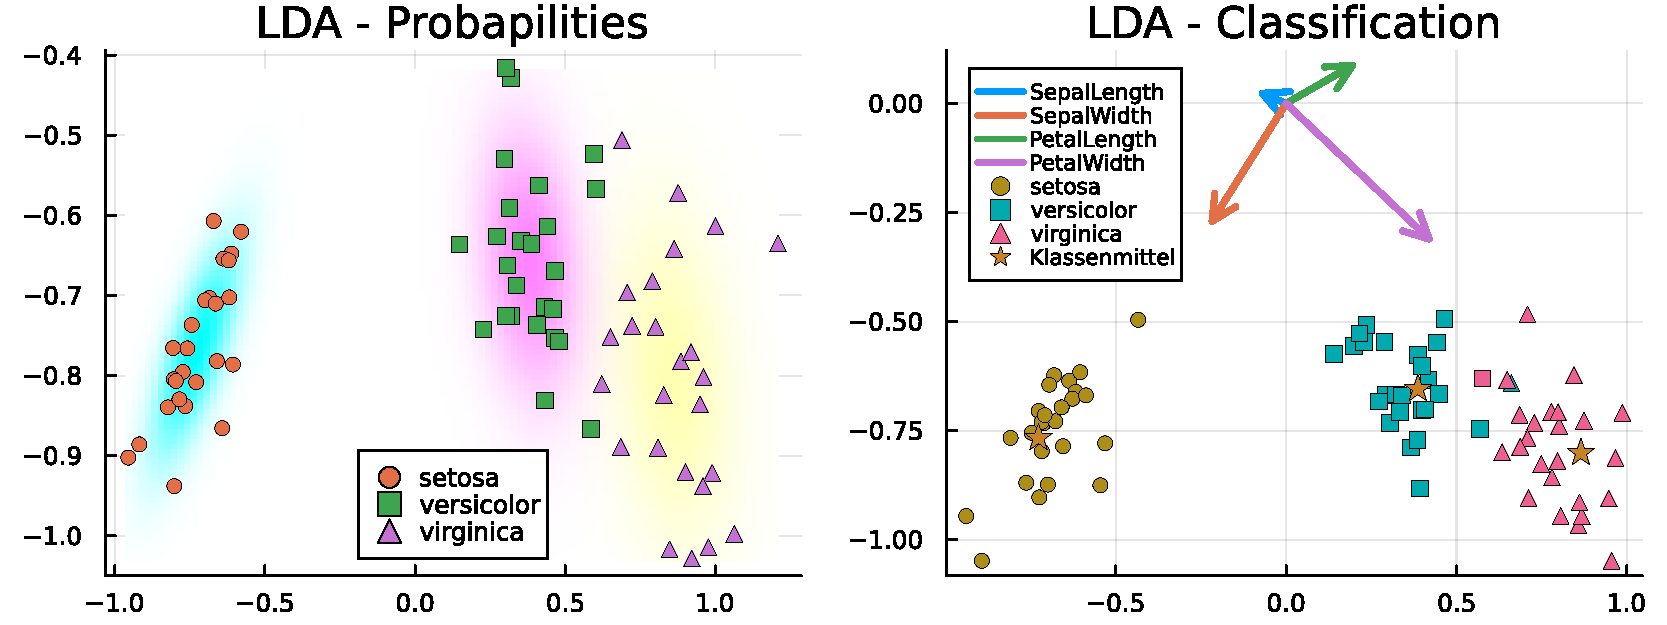
\includegraphics[width=.95\columnwidth]{lda.pdf}
\end{figure}

\subsection{Hauptkomponentenanalyse}

Transformiert in linear unkorrelierte Variablen, wobei die ersten Achsen die
meiste Information enthalten.

\begin{lstlisting}
using MultivariateStats, RDatasets
iris = dataset("datasets", "iris")  # Daten
# Kelchblatt-Sepal, Kronblatt-Petal, Länge/Breite
M = Matrix(iris[1:2:end,1:4])'      # Trainingsdaten
s = iris[1:2:end,5]  # Art setosa virginica versicolor
Mt = Matrix(iris[2:2:end,1:4])'     # Testdaten
st = iris[2:2:end,5]

pca = fit(PCA, M; maxoutdim=2)
pca.prinvars                      # 4.31 0.22; Loadings
pca.tprinvar / pca.tvar      # 0.974; Informationsgehalt
Mtp = predict(pca, Mt)            # Umprojizieren
Mtr = reconstruct(pca, Mtp)       # Zurückprojizieren
sum((Mt .- Mtr).^2) / sum(Mt.^2)  # 0.00143

using StatsBase
#Daten Standardisieren
ZST = fit(ZScoreTransform, M, dims=2)
pcaS = fit(PCA, StatsBase.transform(ZST, M); maxoutdim=2)
MtSp = predict(pcaS, StatsBase.transform(ZST, Mt))

using Plots
shp = [:circle,:rect,:utriangle]
species = unique(s)
p = plot(layout=(1,2), size=(800,300))
proj = pca.proj
for i=1:4
  plot!(p[1], [0,proj[i,1]], [0,proj[i,2]], arrow=true,
    label=names(iris)[i], linewidth=3)
end
for i in 1:3
  j = st .== species[i]
  scatter!(p[1], Mtp[1,j], Mtp[2,j], label=species[i],
   markershape=shp[i])
end
plot!(p[1], legend=:top, legend_columns=2)
plot!(p[1], title="PCA")
proj = pcaS.proj
for i=1:4
  plot!(p[2], [0,proj[i,1]], [0,proj[i,2]], arrow=true,
    label=names(iris)[i], linewidth=3)
end
for i in 1:3
  j = st .== species[i]
  scatter!(p[2], MtSp[1,j], MtSp[2,j], label=species[i],
   markershape=shp[i])
end
plot!(p[2], legend=:bottom, legend_columns=2)
plot!(p[2], title="PCA Standardised")
\end{lstlisting}

\begin{figure}[h]
  \centering
  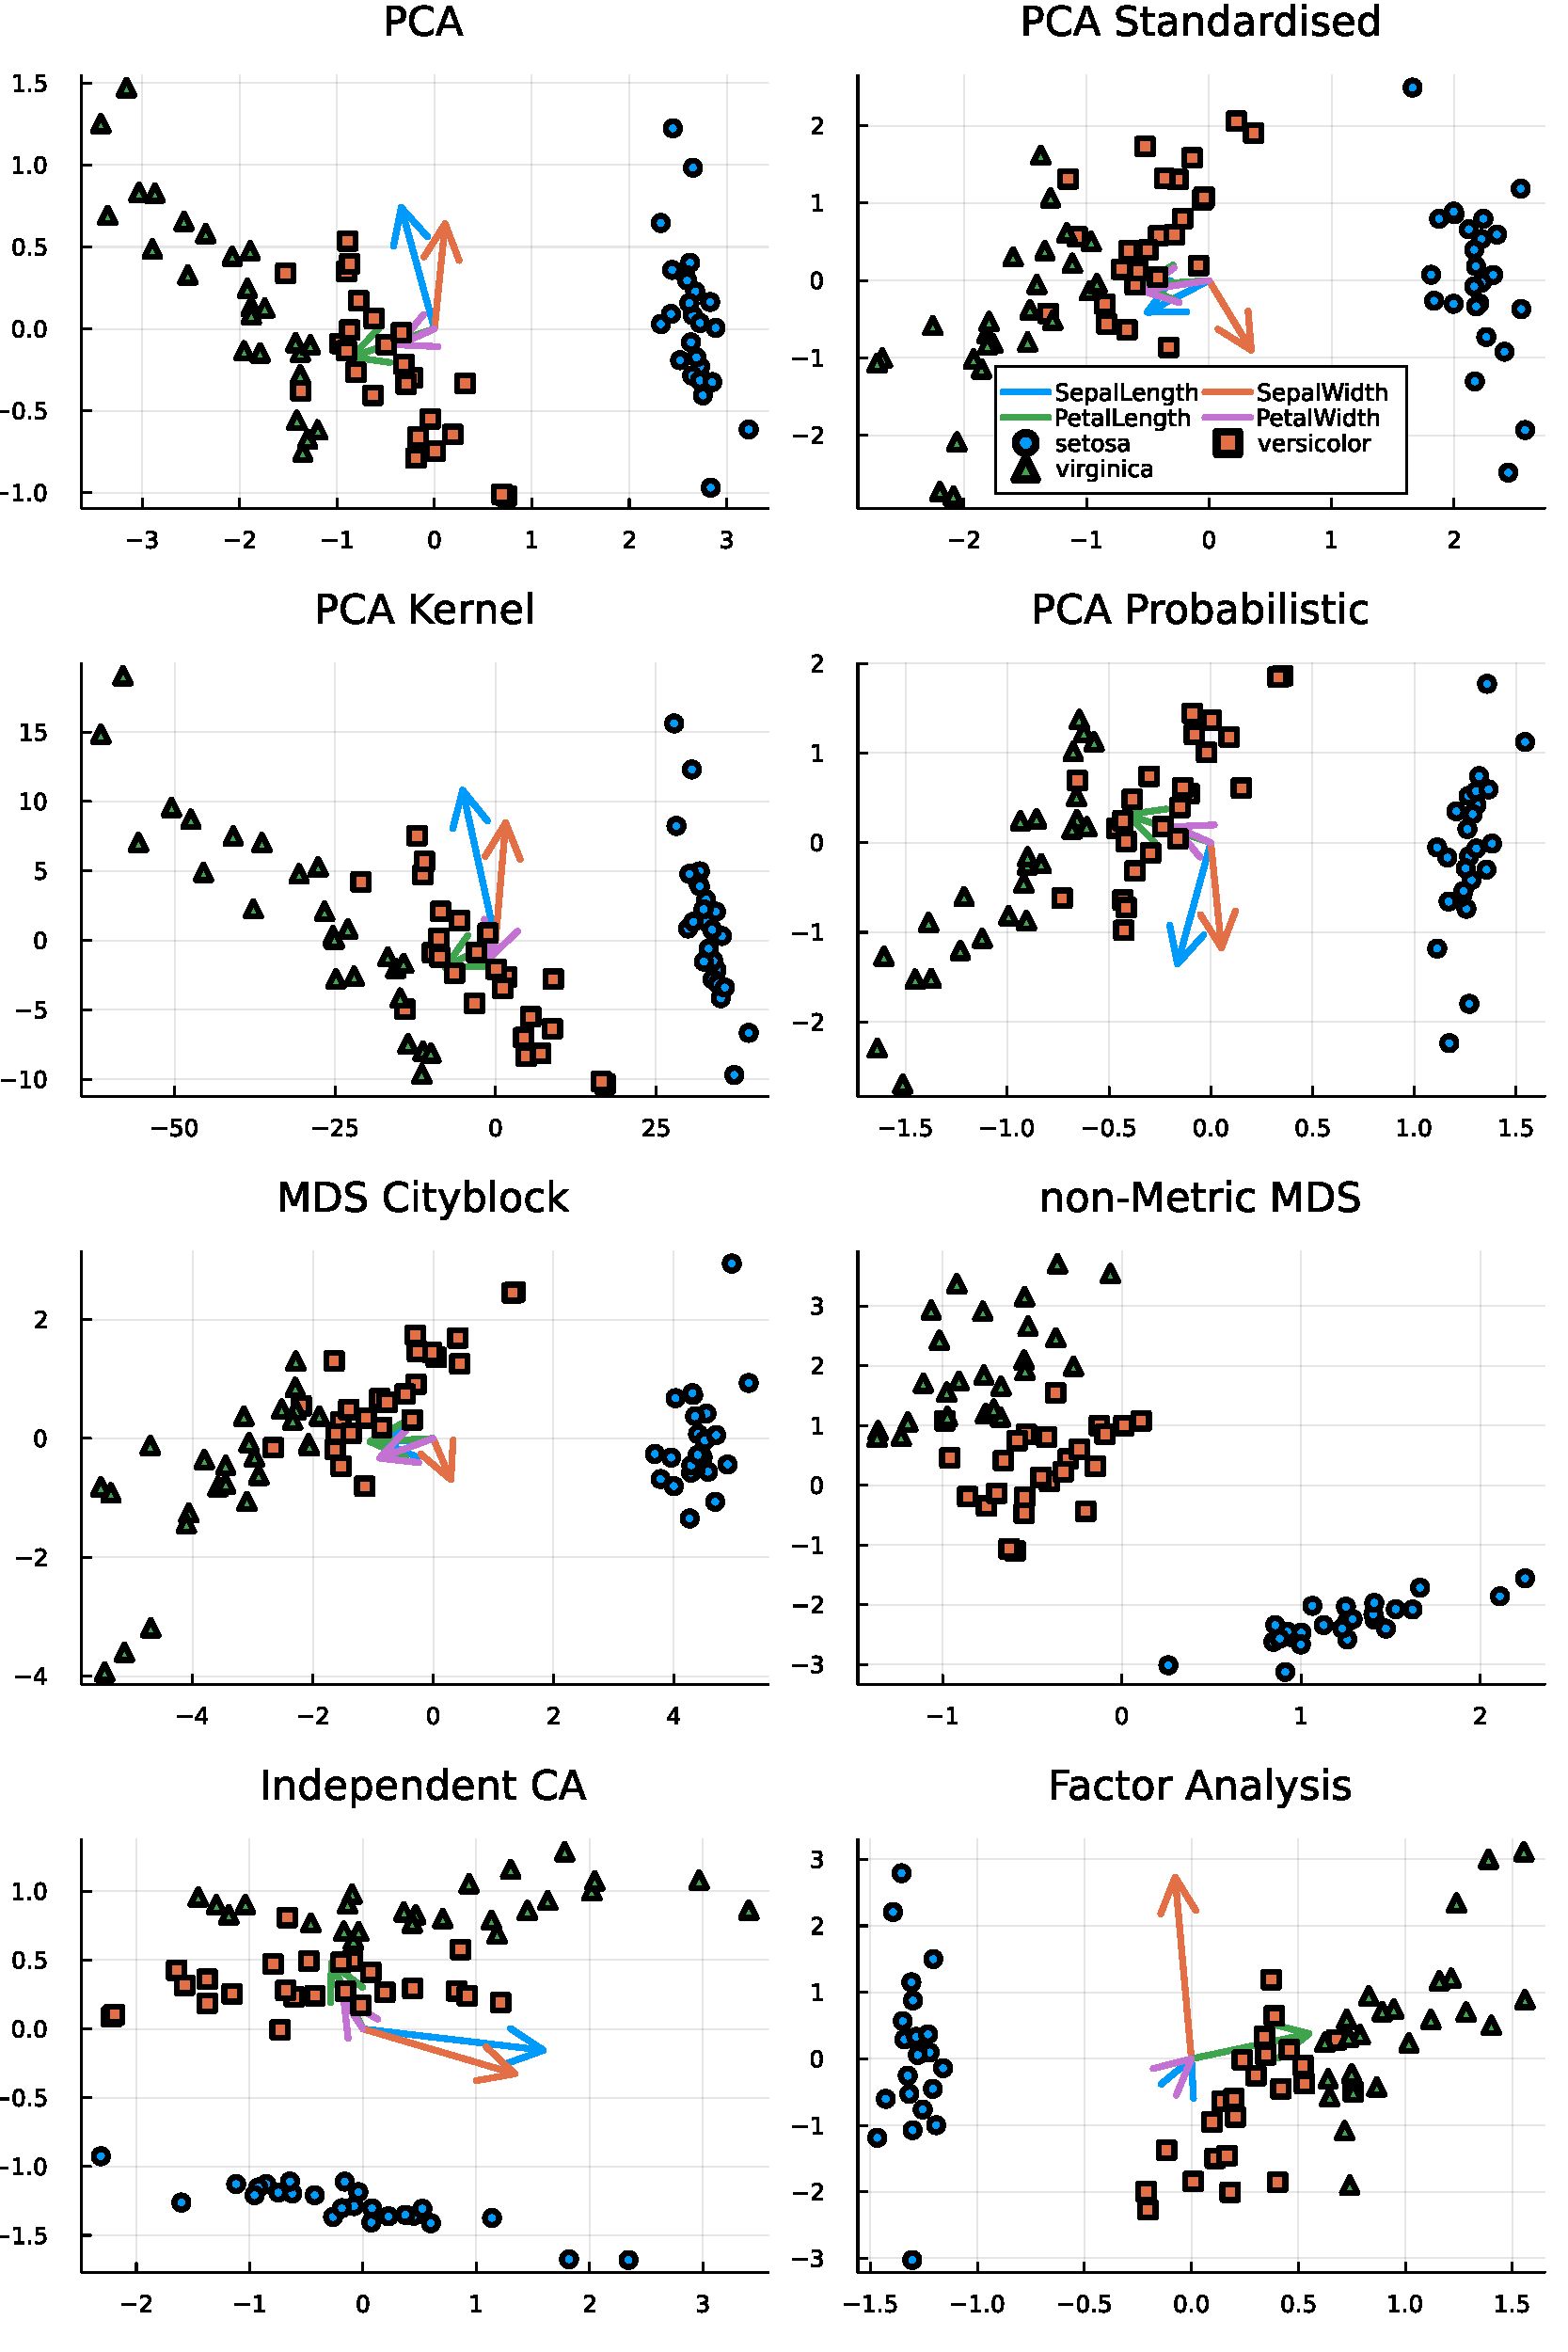
\includegraphics[width=.95\columnwidth]{pca.pdf}
\end{figure}

\section{Clustgering Clusteranalyse}

Version: 0.15.4

\begin{lstlisting}
using RDatasets, Clustering, Plots, Distances
iris = dataset("datasets", "iris"); # load the data
M = Matrix(iris[:, ["SepalWidth", "PetalWidth"]])'
 # Nur zwei Spalten verwenden
s = iris.Species

rKmeans = kmeans(M, 3)  # K-means für 3 Cluster
rKmeans.centers         # Klassenmittel
rKmedoids = kmedoids(pairwise(SqEuclidean(), M), 3)
rHclust = hclust(pairwise(SqEuclidean(), M);
 linkage=:single)
rHclustB = hclust(pairwise(SqEuclidean(), M);
 linkage=:ward_presquared)
rMcl = mcl(pairwise(SqEuclidean(), M))
rAffin = affinityprop(pairwise(SqEuclidean(), M))
rDbscan = dbscan(M, .3, min_neighbors = 3,
 min_cluster_size = 20)
rFuzzy = fuzzy_cmeans(M, 3, 2)

P = function(p, z, T="")
  shp = [:circle,:rect,:utriangle]
  scatter!(p, M[1,:], M[2,:], marker_z=z,
   markershape=shp[s.refs], title=T, color=:lightrainbow)
end 
p = plot(layout=(4,2), size=(800,1200), legend=false)
P(p[1], rKmeans.assignments, "K-Means")
P(p[2], rKmedoids.assignments, "K-Medoids")
P(p[3], cutree(rHclust; k=3),
 "Hierarchical Clustering - Single")
P(p[4], cutree(rHclustB; k=3),
 "Hierarchical Clustering - Ward")
P(p[5], rMcl.assignments, "Markov Cluster Algorithm")
P(p[6], rAffin.assignments, "Affinity propagation")
P(p[7], rDbscan.assignments, "DBSCAN")
P(p[8], getindex.(argmax(rFuzzy.weights, dims = 2), 2),
 "Fuzzy C-means")
savefig("cluster.pdf")
\end{lstlisting}

\begin{figure}[h]
  \centering
  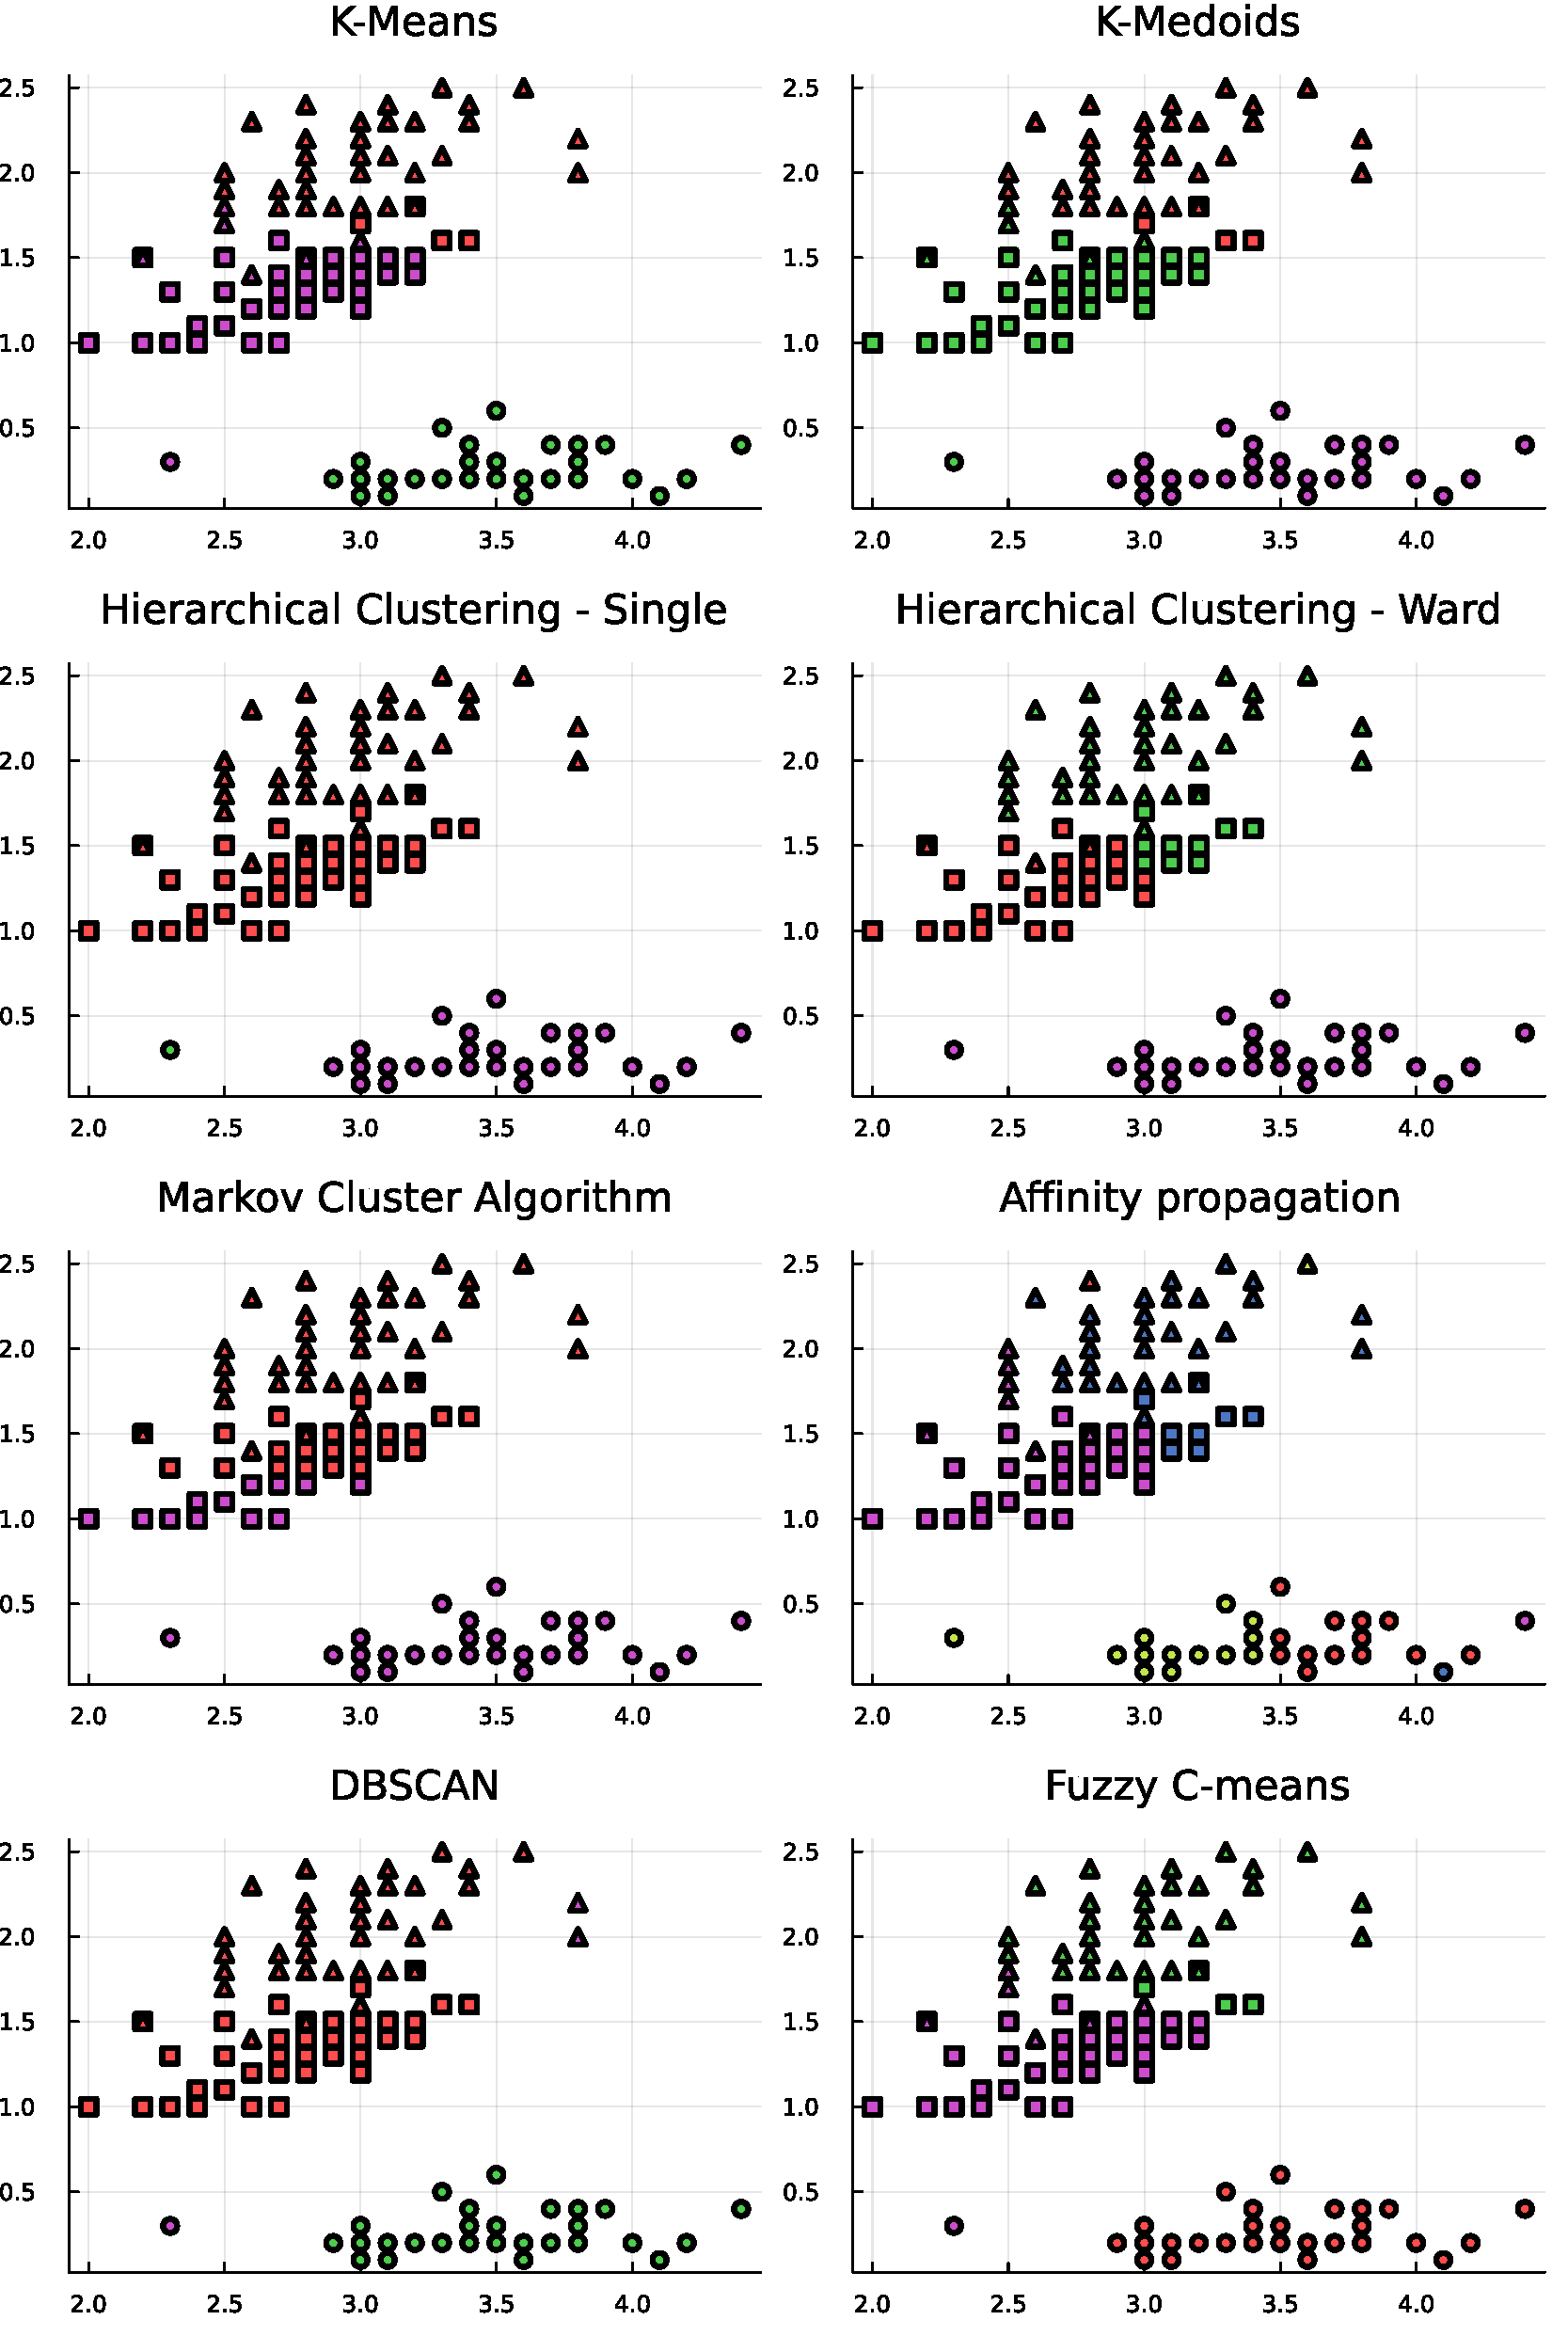
\includegraphics[width=.95\columnwidth]{cluster.pdf}
\end{figure}


\section{Regression}

\subsection{Base}

Koeffizienten von linearen Regressionen können ohne zusätzliche Pakete mit
\lstinline|\| geschätzt werden.

\begin{lstlisting}
X = [[1,1,1,1] [1,2,3,4]]
y=[2,4,7,10]
# y = c[1] * X[:,1] + c[2] * X[:,2]
c = X\y              # -1.0 2.7; Koeffizienten
# y = c[1] * X[:,1] + c[2] * X[:,2] + c[3] * X[:,2]^2
c = [X X[:,2].^2]\y  # 0.25 1.45 0.25
\end{lstlisting}

\subsection{GLM}

Koeffizienten von linearen und verallgemeinerten linearen Modelle können mit
\lstinline|GLM| (Version 1.8.3.) geschätzt werden.

\subsubsection{Linear}

\begin{lstlisting}
using GLM
X = [[1,1,1,1] [1,2,3,4]]
y = [2,4,7,10]
ols = fit(LinearModel, X, y)     # Lineare Regression
ols = lm(X, y)  # Alternative
using DataFrames
data = DataFrame(X=[1,2,3,4], y=[2,4,7,10])
ols = lm(@formula(y ~ X), data)  # Alternative
coeftable(ols)            # Koefizienten mit Signifikanz
ols                              # Alternative
 #             Coef.  Std. Error      t  Pr(>|t|)
 #(Intercept)   -1.0    0.474342  -2.11    0.1695
 #X              2.7    0.173205  15.59    0.0041
  #Lower 95%  Upper 95%
  # -3.04093    1.04093
  #  1.95476    3.44524
coef(ols)          # -1.0 2.7; Koefizienten
coefnames(ols)     # (Intercept) X; Namen
deviance(ols)      # 0.30; Standardaweichung Modell
nulldeviance(ols)  # 36.75; Standardaweichung 0-Modell
fitted(ols)        # 1.7 4.4 7.1 9.8; Modelschätzwerte
predict(ols)       # Modelschätzwerte
predict(ols, DataFrame(X=[0,5]))
 # -1 12.5; Modelschätzwerte mit neuen Daten
response(ols)      # 2 4 7 10; Originalwerte
residuals(ols)     # 0.3 -0.4 -0.1 0.2; Residuen
cooksdistance(ols)
 # 2.3 0.3 0.02 1.0; Einfluss der Datenpunkte
r2(ols)            # 0.992; Korrelation
adjr2(ols)         # 0.988; Adjustierte Korrelation
confint(ols)       # Konfidenzinterval der Koeffizienten
 #-3.04093  1.04093
 # 1.95476  3.44524
stderror(ols)      # Standardfehler der Koeffizienten
 # 0.47 0.17
vcov(ols)   # Varianz-Kovarianz-Matrix der Koeffizienten
 # 0.225  -0.075
 #-0.075   0.03
dof(ols)    # 3; Konsumierte Freiheitsgrade des Modells
nobs(ols)   # 4; Anzahl unabhängiger Beobachtungen
ftest(ols.model)  # Unterschied Modell zu 0-Modell
 # 0.0041; Signifkikant
ols2 = lm(@formula(y ~ X + X^2), data)
ftest(ols.model, ols2.model)  # Unterschied ols zu ols2
 # 0.27; Nicht signifikant
using StatsBase
aic(ols)   # 6.99; Akaike's Information Criterion
aicc(ols)  # Inf; Corrected Akaike's for small samples
bic(ols)   # 5.15; Bayesian Information Criterion

using Plots
p = plot(layout=(1,2), size=(800,300))
scatter!(p[1], data.X, data.y, label="Beobachtung")
Plots.abline!(reverse(coef(ols))..., label="ols")
ND = DataFrame(X=1:.25:4)  # Neue Daten
plot!(p[1], ND.X, predict(ols2, ND), label="ols2")
scatter!(p[2], fitted(ols), residuals(ols), label="ols",
 xlabel="Predicted", ylabel="Residuen")
scatter!(p[2], fitted(ols),residuals(ols2),label="ols2")
savefig("glm.pdf")
\end{lstlisting}

\begin{figure}[h]
  \centering
  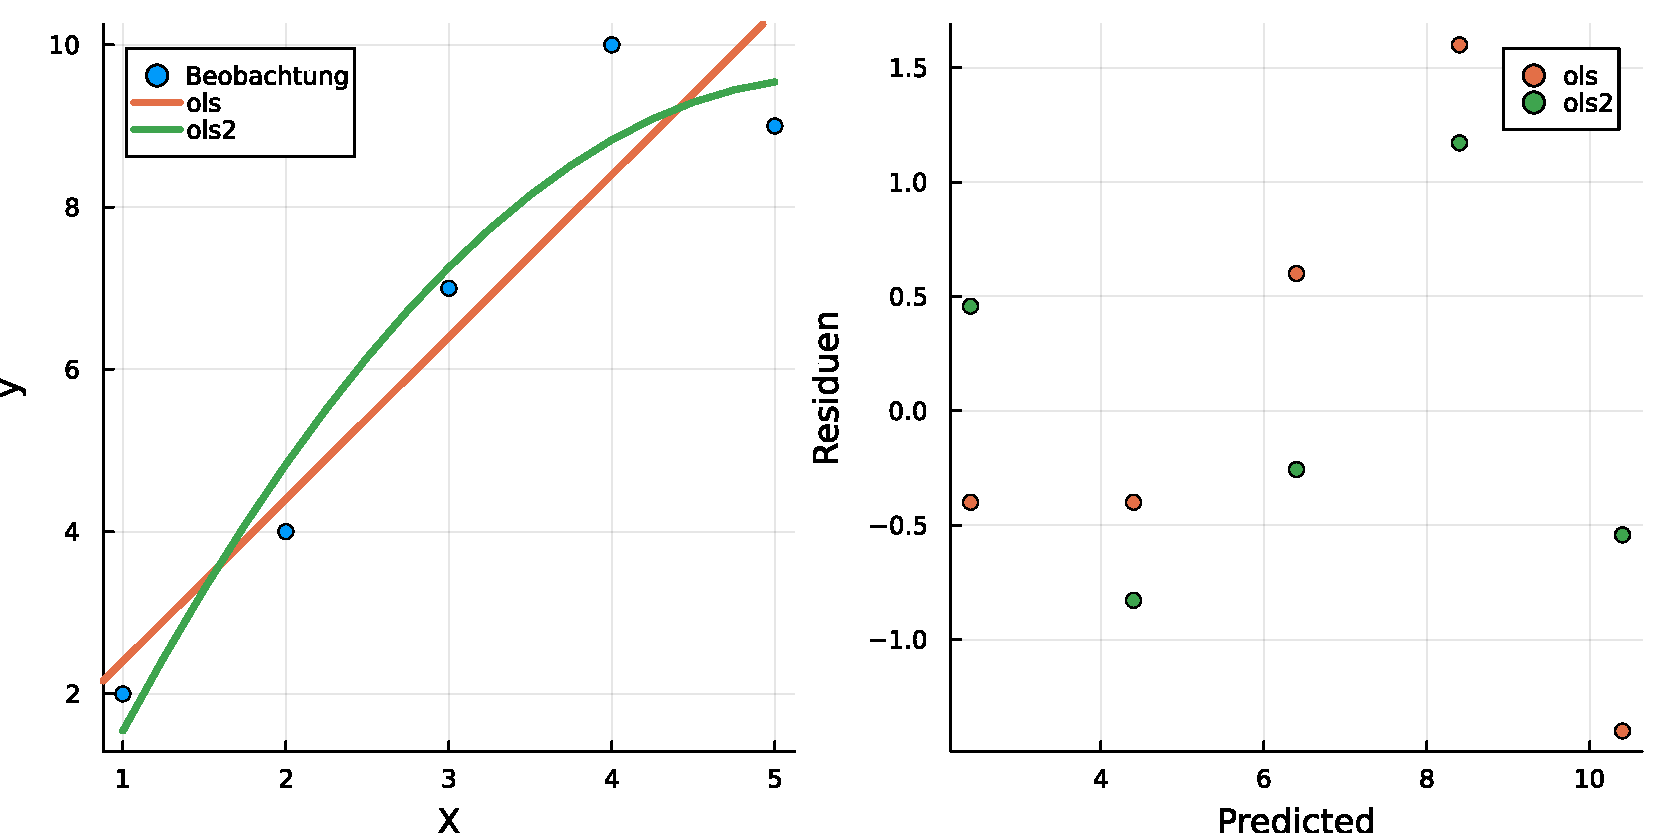
\includegraphics[width=.95\columnwidth]{glm.pdf}
\end{figure}

\subsubsection{Kategoriale Variablen}
\label{ssec:kategorialeVariablen}

Diese werden automatisch als Dummy--Matrix codiert.

\begin{lstlisting}
using GLM, DataFrames
data = DataFrame(X=[1,2,3,4,5], c=["a","a","b","b","b"],
 y=[2,4,7,10,13])
# Intercept und Differenz dazu
ols = lm(@formula(y ~ c), data)
 #(Intercept)    3.0
 #c: b           7.0
# Intercept je Gruppe
ols = lm(@formula(y ~ 0 + c), data)
 #c: a    3.0
 #c: b   10.0
# Intercept Differenz; gemeinsamer Anstieg
ols = lm(@formula(y ~ c + X), data)
 #(Intercept)  -1.2
 #c: b          0.0
 #X             2.8
# Intercept, Anstieg und Differenz dazu
ols = lm(@formula(y ~ c * X), data)
 #(Intercept)   0.0
 #c: b         -2.0
 #X             2.0
 #c: b & X      1.0
# kein Inercept; Anstieg je Gruppe
ols = lm(@formula(y ~ 0 + c & X), data)
 #c: a & X   2.0
 #c: b & X   2.52
# Gemeinsames Intercept; Anstieg je Gruppe
ols = lm(@formula(y ~ c & X), data)
 #(Intercept)  -0.75
 #c: a & X      2.45
 #c: b & X      2.7
# Intercept Differenz; Anstieg je Gruppe
ols = lm(@formula(y ~ c + c & X), data)
 #(Intercept)   0.0
 #c: b         -2.0
 #c: a & X      2.0
 #c: b & X      3.0
# Intercept und Anstieg je Gruppe
ols = lm(@formula(y ~ 0 + c + c & X), data)
 #c: a        0.0
 #c: b       -2.0
 #c: a & X    2.0
 #c: b & X    3.0
\end{lstlisting}

\subsubsection{Generalized Linear}

Für eine GLM muss deren Verteilung (\lstinline|family|) und Funktion
(\lstinline|link|) angegeben werden. Mit \lstinline|?Link| kann man alle verfügbaren Linktypen anzeigen.

\begin{lstlisting}
using GLM, DataFrames

#Binomial Logit Modell
data = DataFrame(X=[1,2,2,3], y=[0,0,1,1])
logit = glm(@formula(y ~ X), data,Binomial(),LogitLink())
logit = glm(@formula(y ~ X), data, Binomial())  # Gleich
1 ./ (1 .+ exp.(-coef(logit)[1].-coef(logit)[2].*data.X))
predict(logit)  # Gleich
#Werte zwischen 0 und 1
data = DataFrame(X=[1,2,3], y=[0,0.5,1])
logit = glm(@formula(y ~ X), data, Binomial())

#Poisson Log Modelldata = DataFrame(X=[1,2,3,4], y=[2,6,20,50])
reg = glm(@formula(y ~ X), data, Poisson(), LogLink())
reg = glm(@formula(y ~ X), data, Poisson())  # Gleich
exp.(coef(reg)[1] .+ coef(reg)[2] .* data.X)
predict(reg)  # Gleich
#Mit anderen Verteilungen
r2 = glm(@formula(y ~ X), data, Gamma(), LogLink())
r3 = glm(@formula(y~X),data,InverseGaussian(),LogLink())
r4 = glm(@formula(y ~ X), data, Normal(), LogLink())
r5 = lm(@formula(log(y) ~ X), data)

using Plots
ND = DataFrame(X=1:0.2:4)
p = plot(layout=(1,2), size=(800,300))
scatter!(p[1], data.X, data.y, label="Beobachtung")
plot!(p[1], ND.X, predict(reg, ND), label="Poisson")
plot!(p[1], ND.X, predict(r2, ND), label="Gamma")
plot!(p[1],ND.X,predict(r3,ND),label="InverseGaussian")
plot!(p[1], ND.X, predict(r4, ND), label="Normal")
plot!(p[1], ND.X, exp.(predict(r5,ND)),
  label="Linearisiert")

scatter!(p[2], data.X, data.y - predict(reg),
 label="Poisson", legend=:bottomleft, ylabel="Residuen")
scatter!(p[2], data.X, data.y-predict(r2), label="Gamma")
scatter!(p[2], data.X, data.y - predict(r3),
 label="InverseGaussian")
scatter!(p[2], data.X, data.y-predict(r4),label="Normal")
scatter!(p[2], data.X, data.y - exp.(predict(r5)),
 label="Linearisiert")
savefig("glmLogLink.pdf")

D1 = DataFrame(X=[1,2,3], y=[0  ,3,7])
D2 = DataFrame(X=[1,2,3], y=[0.1,3,7])
glm(@formula(y ~ X), D1, Poisson(), LogLink())  # OK
#glm(@formula(y ~ X), D2, Poisson(), LogLink())
 # Error wegen 0.1
#glm(@formula(y ~ X), D1, Normal(), LogLink())
 # Error wegen 0
glm(@formula(y ~ X), D2, Normal(), LogLink())   # OK
\end{lstlisting}

\begin{figure}[h]
  \centering
  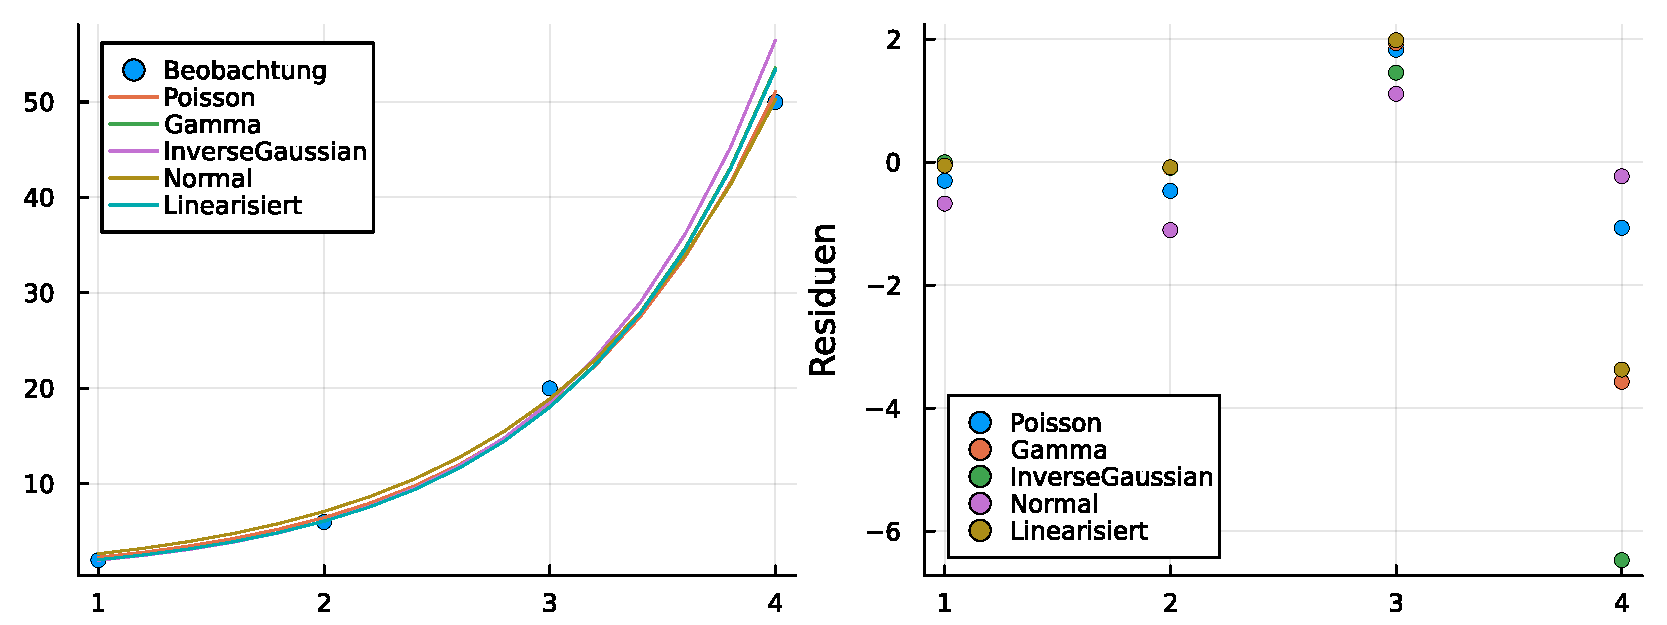
\includegraphics[width=.95\columnwidth]{glmLogLink.pdf}
\end{figure}

\subsubsection{Formular}

Siehe auch \hyperref[ssec:kategorialeVariablen]{Regression/GLM -- Kategoriale
Variablen}

\begin{lstlisting}
y ~ 1 + a + b + c + b&c

~ .. Formula Separator
1 .. Intercept (Automatisch), 0 .. kein Intercept
a, b, c .. Spalten a, b und C
 Falls Spalte nicht Numeric wird sie contrast coded/Dummy
& .. Interaction Term, Modellmatrix für jedes Spaltenpaar

b + c + b&c  ist Equivalent mit  b*c
(a + b) & c  ergibt  a & c  und  b & c

y ~ 1 + a + log(1+a) .. Intercept, Spalte a und log(1+a)
log(y) ~ 1 + a + b .. Transformation der Abhängigen
y ~ 1 + a + protect(1+a) .. Intercept, a und (1+a)

y ~ 1 + a + a&b   Ist Equvalent mit
Term(:y)~ConstantTerm(1) + Term(:a) + Term(:a) & Term(:b)

y ~ 1 + a + b   Ist Equvalent mit
term(:y) ~ foldl(+, term.((1, :a, "b")))
term(:y) ~ sum(term.((1, :a, "b")))
\end{lstlisting}

Mehrere Regressionen mit verschiedenen Spalten können mithilfe einer Schleife
realisiert werden.

\begin{lstlisting}
using DataFrames, GLM
df = DataFrame(reshape(1:40,:,4), ["y","x1","x2","x3"])
#Regression y~x1, y~x2 und y~x3
for x in names(df)[2:end]
  @show lm(term(:y) ~ term(x), df)
end
#Oder über Auswahl der Spalten
for i in 2:ncol(df)
  @show lm([ones(nrow(df)) df[:,i]], df.y)
end
\end{lstlisting}

\subsection{Lasso}

Lasso \lstinline|v0.7.0| (Least absolute shrinkage and selection operator --
kleinster absoluter Reduzierungs-- und Auswahloperator) kann bei der
Variablenauswahl und Regularisierung helfen, um die Vorhersagegenauigkeit und
Interpretierbarkeit zu verbessern.

\begin{lstlisting}
using Lasso, DataFrames, RDatasets
iris = dataset("datasets", "iris")

#Lasso für GLM mit Family=Normal, Link=LogLink
#ridge (α=0), lasso (α=1)
#Für α=0 muss λ angegeben werden
path = fit(LassoPath,
 @formula(SepalLength ~ PetalLength + log(PetalLength) +
                        PetalLength^2 + 1/PetalLength),
 iris, Normal(), LogLink(); α=0.5)
coef(path, AllSeg())   # Koeffizienten des gesamten Pfades
#Koeffizienten wo AICc minimal
coef(path, MinAICc())  # [1] 1.59 [4] 0.0099
coef(path, MinAIC())   # min AIC
coef(path, MinBIC())   # min BIC
#Cross-validation
#nCVfolds=10 Datensatz in 10 zufällige Teile teilen
coef(path, MinCVmse(path, 10))  # minimum mse
coef(path, MinCV1se(path, 10))  # largest λt
#Detailierte Koeffizientenangabe
selectmodel(path.model, MinAICc())
#          Coef.  Std. Error     z  Pr(>|z|)
# x1  1.58654       3.75845   0.42    0.6729
# x2  0.0           2.68277   0.00    1.0000
# x3  0.0           7.57216   0.00    1.0000
# x4  0.00993123    0.140455  0.07    0.9436
# x5  0.0           6.34331   0.00    1.0000
 #  Lower 95%  Upper 95%
 #  -5.77989    8.95298
 #  -5.25813    5.25813
 # -14.8412    14.8412
 #  -0.265355   0.285217
 # -12.4327    12.4327

#Selektiert ein Modell
using Random, MLBase  # Für Kfold in MinCVmse
m = fit(LassoModel,
 @formula(SepalLength ~ PetalLength + log(PetalLength) +
                        PetalLength^2 + 1/PetalLength),
 iris, Normal(), LogLink();
 select=MinCVmse(Kfold(nrow(iris), 10)))

#Als Ausreichend ausgewählt
m = fit(LassoModel,
 @formula(SepalLength ~ PetalLength^2),
 iris, Normal(), LogLink(); select=MinAIC())
coef(m)                         # 1.59 0.00993
#GLM zum Vergleich
glm = fit(GeneralizedLinearModel,
 @formula(SepalLength ~ PetalLength^2),
 iris, Normal(), LogLink())
coef(glm)                       # 1.59 0.0100
std(predict(m) - predict(glm))  # 0.00525
\end{lstlisting}

\subsection{MixedModels}

Gemischte Modelle \lstinline|v4.17.0| differenzieren zwischen festen und
zufälligen Effekten.

\subsubsection{Scalar random effects}

Skalare Zufallseffekte, als Verschiebung des Intercepts je Gruppe
\lstinline|G|, werden mit \lstinline"(1|G)" in \lstinline|@formula|
angegeben.

\begin{lstlisting}
using MixedModels
dyestuff = MixedModels.dataset(:dyestuff)  # Daten
#Zufallsefekt von batch mit Intercept bereücksichtigen
fm = @formula(yield ~ (1|batch))  # Intercept automatisch
fm = @formula(yield ~ 1 + (1|batch))  # Gleich
fm1 = fit(MixedModel, fm, dyestuff)  # maximum likelihood
fm1reml = fit(MixedModel, fm, dyestuff, REML=true) # REML

fm1.beta  # 1527.5; Fixe effekte
coef(fm1)
fixef(fm1)
coeftable(fm1)  # Als Tabelle
 #              Coef.  Std. Error      z  Pr(>|z|)
 #(Intercept)  1527.5     17.6946  86.33    <1e-99

fm1.b  # Zufallsefekte
 #-16.63  0.37  26.97  -21.8  53.58  -42.49
ranef(fm1)
only(raneftables(fm1))  # Als Tabelle

#Zum Vergleich Mittel und Median
using DataFrames, Statistics, GLM
d = DataFrame(dyestuff)
m = mean(d.yield)
LM = lm(@formula(yield ~ 0 + batch), d)
md = median(d.yield)
gd = combine(groupby(d, :batch), :yield => median)
["Modell\batch" "fix" permutedims(unique(dyestuff.batch))
"MMMaxLi" fm1.beta round.(ranef(fm1)[1]; digits=1)
"MMReml" fm1reml.beta round.(ranef(fm1reml)[1]; digits=1)
"lm mean" m (coef(LM) .- m)'
"median" md (gd[:,2] .- md)']
 # "Modell\batch"      "fix"     "A"    "B"    "C"
 # "MMMaxLi"       1527.5     -16.6    0.4   27.0
 # "MMReml"        1527.5     -17.6    0.4   28.6
 # "lm mean"       1527.5     -22.5    0.5   36.5
 # "median"        1530.0     -10.0   10.0   30.0
  #    "D"    "E"     "F"
  # -21.8   53.6   -42.5
  # -23.1   56.7   -45.0
  # -29.5   72.5   -57.5
  # -65.0   95.0   -75.0
\end{lstlisting}

Mehrere Gruppen werden mit \lstinline|+| verbunden: \lstinline"(1|G) + (1|H)".

\begin{lstlisting}
using MixedModels
penicillin = MixedModels.dataset(:penicillin)
fm3 = fit(MixedModel, @formula(diameter ~ 1 + (1|plate) +
    (1|sample)), penicillin)
fixef(fm3)  # 22.97
raneftables(fm3)[1]
#    plate  (Intercept)
#1 | a      0.804403
#2 | b      0.804403
#: | :         :
raneftables(fm3)[2]
#    sample  (Intercept)
#1 | A       2.18566
#2 | B       -1.00983
#: | :         :
\end{lstlisting}

Bei hierarchischer (nested) Gruppierung wird \lstinline|/| verwendet:
\lstinline"(1|G/H)", wobei \lstinline|H| Untergruppen sind, die in \lstinline|G|
enthalten sind. Wenn die Bezeichnungen (levels) der inneren Gruppe
ausschließlich (unique) in der ihr übergeordneten Gruppe zu finden sind, muss
diese Verschachtelung nicht explizit in der Modellsyntax ausgedrückt werden und
kann dann auch mit \lstinline"(1|G) + (1|H)" beschrieben werden.

\begin{lstlisting}
using MixedModels, DataFrames
pastes = DataFrame(MixedModels.dataset(:pastes))
fm4a = fit(MixedModel, @formula(strength ~ 1 +
 (1|batch/cask)), pastes)
pastes.sample = (string.(pastes.batch, "&", pastes.cask))
fm4b = fit(MixedModel, @formula(strength ~ 1 +
 (1|sample) + (1|batch)), pastes)
fixef(fm4a)  # 60.05
fixef(fm4b)  # 60.05
raneftables(fm4a)[1]
#    batch & cask  (Intercept)
#1 | ("A", "a")    1.92557
#2 | ("A", "b")    0.483539
#: |      :         :
raneftables(fm4b)[1]
#   sample  (Intercept)
#1 | A&a     1.92557
#2 | A&b     0.483539
#: |      :         :
raneftables(fm4a)[2]
#    batch  (Intercept)
#1 | A      0.643691
#2 | B      -0.219088
#: |      :         :
raneftables(fm4b)[2]
#    batch  (Intercept)
#1 | A      0.643691
#2 | B      -0.219088
#: |      :         :
\end{lstlisting}

\subsubsection{Vector--valued random effects}

Vektorwert Zufallseffekte, als Veränderung des Anstiegs von \lstinline|X| je
Gruppe \lstinline|G|, werden mit \lstinline"(X|G)" in \lstinline|@formula|
angegeben. Mit \lstinline"(1 + X|G)" wird sowohl Intercept als auch Anstieg je
Gruppe angepasst. Wobei hier auch die Korrelation zwischen den Zufallseffekten
für verschiedene Prädiktoren bestimmt wird. Diese Korrelation wird nicht
bestimmt (z.\~B.\ gewünscht wenn viele Zufallsefekte vorhanden sind) wenn
\lstinline"(1|G) + (X|G)" oder \lstinline"zerocorr(1 + days|subj)" verwendet
wird.

\begin{lstlisting}
using MixedModels
sleepstudy = MixedModels.dataset(:sleepstudy)
fm2 = fit(MixedModel, @formula(reaction ~ 1 + days +
 (1 + days|subj)), sleepstudy)
VarCorr(fm2)
#Variance components:
#            Column    Variance Std.Dev.   Corr.
#subj     (Intercept)  565.51068 23.78047
#         days          32.68212  5.71683 +0.08
#Residual              654.94145 25.59182
coeftable(fm2)
#                Coef.  Std. Error      z  Pr(>|z|)
#(Intercept)  251.405      6.63226  37.91    <1e-99
#days          10.4673     1.50224   6.97    <1e-11
only(raneftables(fm2))
#    subj  (Intercept)  days
#1 | S308    2.81582     9.07551
#2 | S309  -40.0484     -8.64408
#3 | S310  -38.4331     -5.5134
#: |  :         :           :

fm2b = fit(MixedModel, @formula(reaction ~ 1 + days +
 (1|subj) + (days|subj)), sleepstudy)
VarCorr(fm2b)
#Variance components:
#            Column    Variance Std.Dev.   Corr.
#subj     (Intercept)  584.25897 24.17145
#         days          33.63281  5.79938   .
#Residual              653.11578 25.55613
coeftable(fm2b)
#                Coef.  Std. Error      z  Pr(>|z|)
#(Intercept)  251.405      6.70771  37.48    <1e-99
#days          10.4673     1.51931   6.89    <1e-11
only(raneftables(fm2b))
#    subj  (Intercept)  days
#1 | S308  1.85472      9.23642
#2 | S309  -40.0225     -8.61744
#3 | S310  -38.7233     -5.43435
#: |  :         :           :
\end{lstlisting}

Bei qualitativen Prediktoren werden Korrelationen zwischen allen Ausprägungen (Levels) geschätzt. Mit \lstinline|zerocorr| und \lstinline|fulldummy| kann dies verhindert werden.

\begin{lstlisting}
using MixedModels
sleepstudy = MixedModels.dataset(:sleepstudy)

#Korrelation zwischen jedem Level und auch Intercept
fm2c = fit(MixedModel, @formula(reaction ~ 1 + days +
 (1 + days|subj)), sleepstudy,
    contrasts = Dict(:days => DummyCoding()))
VarCorr(fm2c)
#Variance components:
#            Column    Variance  Std.Dev.   Corr.
#subj     (Intercept)   955.69001 30.91424
#         days: 1       493.28331 22.20998 -0.30
#         days: 2       911.69517 30.19429 -0.57 +0.75
#            :              :        :
coeftable(fm2c)
#(Intercept)  256.652       7.36615  34.84    <1e-99
#days: 1        7.84395     5.45319   1.44    0.1503
#days: 2        8.71009     7.2789    1.20    0.2315
#   :            :           :         :       :
only(raneftables(fm2c))
#     subj  (Intercept)  days: 1   days: 2   days: 3 ...
# 1 | S308  -7.72997     3.81182   -7.1743   46.5738 ...
# 2 | S309  -34.3748     -24.2256  -27.2167  -43.7698...
#   :   :   :

#Keine Korrelation
fm2d = fit(MixedModel, @formula(reaction ~ 1 + days +
 zerocorr(1 + fulldummy(days)|subj)), sleepstudy,
    contrasts = Dict(:days => DummyCoding()))
VarCorr(fm2d)
#Variance components:
#            Column     Variance    Std.Dev.    Corr.
#subj     (Intercept)  1135.1084091 33.6913700
#         days: 0       775.8089921 27.8533480   .
#         days: 1       357.6378321 18.9113149   . .
#         days: 2       221.0775456 14.8686767   . . .
#            :              :        :
coeftable(fm2d)
#                 Coef.  Std. Error      z  Pr(>|z|)
#(Intercept)  256.652      10.7804   23.81    <1e-99
#days: 1        7.84395     9.11488   0.86    0.3895
#days: 2        8.71009     8.68874   1.00    0.3161
#   :            :           :         :       :
only(raneftables(fm2d))
#     subj  (Intercept)  days: 0   days: 1   days: 2 ...
# 1 | S308  35.4252      -34.4738  -27.366   -27.4841...
# 2 | S309  -73.5839     32.1622   9.53044   6.15799 ...
#   :   :   :
\end{lstlisting}

Für eine GLMM muss deren Verteilung (\lstinline|family|) und bei Bedarf die
Funktion (\lstinline|link|) angegeben werden. Mit \lstinline|fast=true|, kann eine schnellere, aber etwas ungenauere Anpassung erfolgen.

\begin{lstlisting}
using MixedModels
verbagg = MixedModels.dataset(:verbagg)
gm = fit(MixedModel, @formula(r2 ~ 1 + anger + (1|subj)),
         verbagg, Bernoulli(), LogitLink())
gm2 = fit(MixedModel, @formula(r2 ~ 1 + anger + (1|subj)),
          verbagg, Bernoulli(), LogitLink(), fast=true)

\end{lstlisting}



%Autor: Georg Kindermann

\end{document}
